% 2-15-rb-tree.tex

%%%%%%%%%%%%%%%%%%%%
\documentclass[a4paper, justified]{tufte-handout}

% hw-preamble.tex

% geometry for A4 paper
% See https://tex.stackexchange.com/a/119912/23098
\geometry{
  left=20.0mm,
  top=20.0mm,
  bottom=20.0mm,
  textwidth=130mm, % main text block
  marginparsep=5.0mm, % gutter between main text block and margin notes
  marginparwidth=50.0mm % width of margin notes
}

% for colors
\usepackage{xcolor} % usage: \color{red}{text}
% predefined colors
\newcommand{\red}[1]{\textcolor{red}{#1}} % usage: \red{text}
\newcommand{\blue}[1]{\textcolor{blue}{#1}}
\newcommand{\teal}[1]{\textcolor{teal}{#1}}

\usepackage{todonotes}

% heading
\usepackage{sectsty}
\setcounter{secnumdepth}{2}
\allsectionsfont{\centering\huge\rmfamily}

% for Chinese
\usepackage{xeCJK}
\usepackage{zhnumber}
\setCJKmainfont[BoldFont=FandolSong-Bold.otf]{FandolSong-Regular.otf}

% for fonts
\usepackage{fontspec}
\newcommand{\song}{\CJKfamily{song}} 
\newcommand{\kai}{\CJKfamily{kai}} 

% To fix the ``MakeTextLowerCase'' bug:
% See https://github.com/Tufte-LaTeX/tufte-latex/issues/64#issuecomment-78572017
% Set up the spacing using fontspec features
\renewcommand\allcapsspacing[1]{{\addfontfeature{LetterSpace=15}#1}}
\renewcommand\smallcapsspacing[1]{{\addfontfeature{LetterSpace=10}#1}}

% for url
\usepackage{hyperref}
\hypersetup{colorlinks = true, 
  linkcolor = teal,
  urlcolor  = teal,
  citecolor = blue,
  anchorcolor = blue}

\newcommand{\me}[4]{
    \author{
      {\bfseries 姓名:}\underline{#1}\hspace{2em}
      {\bfseries 学号:}\underline{#2}\hspace{2em}\\[10pt]
      {\bfseries 评分:}\underline{#3\hspace{3em}}\hspace{2em}
      {\bfseries 评阅:}\underline{#4\hspace{3em}}
  }
}

% Please ALWAYS Keep This.
\newcommand{\noplagiarism}{
  \begin{center}
    \fbox{\begin{tabular}{@{}c@{}}
      请独立完成作业,不得抄袭。\\
      若得到他人帮助, 请致谢。\\
      若参考了其它资料,请给出引用。\\
      鼓励讨论,但需独立书写解题过程。
    \end{tabular}}
  \end{center}
}

\newcommand{\goal}[1]{
  \begin{center}{\fcolorbox{blue}{yellow!60}{\parbox{0.50\textwidth}{\large 
    \begin{itemize}
      \item 体会``思维的乐趣''
      \item 初步了解递归与数学归纳法 
      \item 初步接触算法概念与问题下界概念
    \end{itemize}}}}
  \end{center}
}

% Each hw consists of four parts:
\newcommand{\beginrequired}{\hspace{5em}\section{作业 (必做部分)}}
\newcommand{\beginoptional}{\section{作业 (选做部分)}}
\newcommand{\beginot}{\section{Open Topics}}
\newcommand{\begincorrection}{\section{订正}}
\newcommand{\beginfb}{\section{反馈}}

% for math
\usepackage{amsmath, mathtools, amsfonts, amssymb}
\newcommand{\set}[1]{\{#1\}}

% define theorem-like environments
\usepackage[amsmath, thmmarks]{ntheorem}

\theoremstyle{break}
\theorempreskip{2.0\topsep}
\theorembodyfont{\song}
\theoremseparator{}
\newtheorem{problem}{题目}[subsection]
\renewcommand{\theproblem}{\arabic{problem}}
\newtheorem{ot}{Open Topics}

\theorempreskip{3.0\topsep}
\theoremheaderfont{\kai\bfseries}
\theoremseparator{:}
\theorempostwork{\bigskip\hrule}
\newtheorem*{solution}{解答}
\theorempostwork{\bigskip\hrule}
\newtheorem*{revision}{订正}

\theoremstyle{plain}
\newtheorem*{cause}{错因分析}
\newtheorem*{remark}{注}

\theoremstyle{break}
\theorempostwork{\bigskip\hrule}
\theoremsymbol{\ensuremath{\Box}}
\newtheorem*{proof}{证明}

% \newcommand{\ot}{\blue{\bf [OT]}}

% for figs
\renewcommand\figurename{图}
\renewcommand\tablename{表}

% for fig without caption: #1: width/size; #2: fig file
\newcommand{\fig}[2]{
  \begin{figure}[htbp]
    \centering
    \includegraphics[#1]{#2}
  \end{figure}
}
% for fig with caption: #1: width/size; #2: fig file; #3: caption
\newcommand{\figcap}[3]{
  \begin{figure}[htbp]
    \centering
    \includegraphics[#1]{#2}
    \caption{#3}
  \end{figure}
}
% for fig with both caption and label: #1: width/size; #2: fig file; #3: caption; #4: label
\newcommand{\figcaplbl}[4]{
  \begin{figure}[htbp]
    \centering
    \includegraphics[#1]{#2}
    \caption{#3}
    \label{#4}
  \end{figure}
}
% for margin fig without caption: #1: width/size; #2: fig file
\newcommand{\mfig}[2]{
  \begin{marginfigure}
    \centering
    \includegraphics[#1]{#2}
  \end{marginfigure}
}
% for margin fig with caption: #1: width/size; #2: fig file; #3: caption
\newcommand{\mfigcap}[3]{
  \begin{marginfigure}
    \centering
    \includegraphics[#1]{#2}
    \caption{#3}
  \end{marginfigure}
}

\usepackage{fancyvrb}

% for algorithms
\usepackage[]{algorithm}
\usepackage[]{algpseudocode} % noend
% See [Adjust the indentation whithin the algorithmicx-package when a line is broken](https://tex.stackexchange.com/a/68540/23098)
\newcommand{\algparbox}[1]{\parbox[t]{\dimexpr\linewidth-\algorithmicindent}{#1\strut}}
\newcommand{\hStatex}[0]{\vspace{5pt}}
\makeatletter
\newlength{\trianglerightwidth}
\settowidth{\trianglerightwidth}{$\triangleright$~}
\algnewcommand{\LineComment}[1]{\Statex \hskip\ALG@thistlm \(\triangleright\) #1}
\algnewcommand{\LineCommentCont}[1]{\Statex \hskip\ALG@thistlm%
  \parbox[t]{\dimexpr\linewidth-\ALG@thistlm}{\hangindent=\trianglerightwidth \hangafter=1 \strut$\triangleright$ #1\strut}}
\makeatother

% for footnote/marginnote
% see https://tex.stackexchange.com/a/133265/23098
\usepackage{tikz}
\newcommand{\circled}[1]{%
  \tikz[baseline=(char.base)]
  \node [draw, circle, inner sep = 0.5pt, font = \tiny, minimum size = 8pt] (char) {#1};
}
\renewcommand\thefootnote{\protect\circled{\arabic{footnote}}} % feel free to modify this file
%%%%%%%%%%%%%%%%%%%%
\title{第4-7讲: 代数编码}
\me{朱宇博}{191220186}{}{}
\date{\zhtoday} % or like 2019年9月13日
%%%%%%%%%%%%%%%%%%%%
\begin{document}
\maketitle
%%%%%%%%%%%%%%%%%%%%
\noplagiarism % always keep this line
%%%%%%%%%%%%%%%%%%%%
\begin{abstract}
  % \begin{center}{\fcolorbox{blue}{yellow!60}{\parbox{0.65\textwidth}{\large 
  %   \begin{itemize}
  %     \item 
  %   \end{itemize}}}}
  % \end{center}
\end{abstract}
%%%%%%%%%%%%%%%%%%%%
\beginrequired

%%%%%%%%%%%%%%%
\begin{problem}[TJ 8-6(b,d)]
best situation?
\end{problem}

\begin{solution}
(b)\\
最小距离为$d_{min}(100011, 110011)=1$\\
best situation: 发出编码(000000),他与其他编码的最小距离最大,为3。故可检测2位错或纠正1位错。\\
(d)\\
最小距离为$d_{min}(0111100, 0110110)=2$\\
best situation: 发出编码(1110000) 或 (1111111) 或 (0001111) 或(0000000),他与其他编码的最小距离最大,为3。故可检测2位错或纠正1位错。\\
\end{solution}
%%%%%%%%%%%%%%%

%%%%%%%%%%%%%%%
\begin{problem}[TJ 8-7(c,d)]
\end{problem}

\begin{solution}
(c)\\
null space: (00100),(00000),(11001),(11101),(11110),(11010),(00111),(00011)\\
type:(5,3)-block\\
generator matrices:\\
 $$\begin{pmatrix}0&1&1\\
			   0&1&1\\
			   1&0&0\\
			   0&1&0\\
			   0&0&1
     \end{pmatrix}$$
      $$\begin{pmatrix}1&0&1\\
			   1&0&1\\
			   0&1&0\\
			   0&0&1\\
			   1&0&0
     \end{pmatrix}$$
因此不唯一\\
(d)\\
null space:
\begin{figure}[htbp]
    \centering
    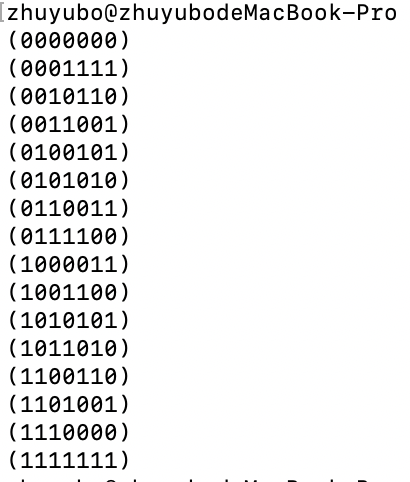
\includegraphics[width = 0.30\linewidth]{figs/a}
  \end{figure}  
\noindent type: (7,4)-block

generator matrices:\\
 $$\begin{pmatrix}1&0&0&0\\
			   0&1&0&0\\
			   0&0&1&0\\
			   0&0&0&1\\
			   0&1&1&1\\
			   1&0&1&1\\
			   1&1&0&1
     \end{pmatrix}$$
     $$\begin{pmatrix}1&0&0&0\\
			   0&1&0&0\\
			   0&0&0&1\\
			    0&0&1&0\\
			   0&1&1&1\\
			   1&0&1&1\\
			   1&1&0&1
     \end{pmatrix}$$因此不唯一\\
\end{solution}
%%%%%%%%%%%%%%%

%%%%%%%%%%%%%%%
\begin{problem}[TJ 8-9]
\end{problem}

\begin{solution}
$H(01111)^T=(001)^T$, so $(01111)\to (01101)$\\
$H(10101)^T=(110)^T$, so Multiple errors\\
$H(01110)^T=(110)^T$, so Multiple errors\\
$H(00011)^T=(110)^T$, so Multiple errors\\
\end{solution}
%%%%%%%%%%%%%%%

%%%%%%%%%%%%%%%
\begin{problem}[TJ 8-11(b,d)]
\end{problem}

\begin{solution}
(b)\\
This is canonical parity-check matrix.\\
corresponding standard generator matrices:\\
 $$\begin{pmatrix}
   			   1&0\\
			   0&1\\
			   0&1\\
			   1&1\\
			   0&1\\
			   1&1\\
     \end{pmatrix}$$
\noindent 可至少纠错一位、检测2位。\\
(d)\\
This is canonical parity-check matrix.\\
corresponding standard generator matrices:\\
 $$\begin{pmatrix}
 1&0&0\\
			   0&1&0\\
			   0&0&1\\0&0&0\\
			   0&1&1\\
			   1&0&1\\
			   0&1&1\\
     \end{pmatrix}$$   
\noindent 可检测一位错,不可纠错。\\
\end{solution}
%%%%%%%%%%%%%%%

%%%%%%%%%%%%%%%
\begin{problem}[TJ 8-13]
\end{problem}

\begin{solution}
(a)$(001)^T$\\
(b)$(101)^T$\\
(c)$(111)^T$\\
(d)$(011)^T$\\
\end{solution}
%%%%%%%%%%%%%%%

%%%%%%%%%%%%%%%
\begin{problem}[TJ 8-19]
\end{problem}

\begin{solution}
(1)群$C$中权重都为奇数。\\
因为$e\in C\land w(e)=0$,显然不成立。\\
(2)群$C$中权重都为偶数。\\
考虑群$C=\{e\}$,此时显然成立,故存在权重都为偶数的情况。\\
(3)群$C$中权重有奇有偶。\\
考虑$c\in C_{odd}$,构造函数$f:C_{even}\to C_{odd}$ by $x\to x+c$其中$x\in C_{even}$(显然$x+c\in C_{odd}$)。\\
one to one:\\
$\forall x_1, x_2\in C_{even}, x_1+ c = x_2 + c \to x_1 = x_2$(right and left cancellation laws in groups)\\
onto:\\
$\forall y\in C_{odd}, \exists x = y + c^{-1}\in C_{even}, st.x + c = y$\\
So $|C_{even}|=|C_{odd}|$, and then exactly half of them have even weight.\\

\noindent Therefore, either every codeword has even weight or exactly half of the codewords have even weight.
\end{solution}
%%%%%%%%%%%%%%%

%%%%%%%%%%%%%%%
\begin{problem}[TJ 8-21]
\end{problem}

\begin{solution}
(a)error-correcting linear code\\
假设$H$矩阵为$m\times n$的,对$2^7=128$进行编码时,需要满足
$$ \left\{
\begin{aligned}
n-m =  7 \\
n \leq 2^ m - 1 \\
\end{aligned}
\right.
$$
$m=4,n=11$为符合条件的最小正整数解。则最小的generator matrix为$11\times 7$。\\
同理,当对$2^8=256$进行编码时,需要满足
$$ \left\{
\begin{aligned}
n-m =  8 \\
n \leq 2^ m - 1 \\
\end{aligned}
\right.
$$
$m=4,n=12$为符合条件的最小正整数解。则最小的generator matrix为$12\times 8$。\\

\noindent(b)only error detection\\
假设$H$矩阵为$m\times n$的,对$2^7=128$进行编码时,需要满足
$$ \left\{
\begin{aligned}
n-m =  7 \\
n \geq 1 \\
\end{aligned}
\right.
$$
$m=1,n=8$为符合条件的最小正整数解。则最小的generator matrix为$8\times 7$。\\
同理,当对$2^8=256$进行编码时,需要满足
$$ \left\{
\begin{aligned}
n-m =  8 \\
n \geq 1 \\
\end{aligned}
\right.
$$
$m=1,n=9$为符合条件的最小正整数解。则最小的generator matrix为$9\times 8$。\\
\end{solution}
%%%%%%%%%%%%%%%

%%%%%%%%%%%%%%%
\begin{problem}[TJ 8-22]
\end{problem}

\begin{solution}
(1)three information position:\\
 $$H=\begin{pmatrix}1&1&1&1\\
 \end{pmatrix}$$
 $$G=\begin{pmatrix}1&0&0\\
			   0&1&0\\
			   0&0&1\\
			   1&1&1\\
 \end{pmatrix}$$
 
 \noindent (2)seven information position:\\
  $$H=\begin{pmatrix}1&1&1&1&1&1&1&1\\
 \end{pmatrix}$$
 $$G=\begin{pmatrix}1&0&0&0&0&0&0\\
			   0&1&0&0&0&0&0\\
			   0&0&1&0&0&0&0\\
			   0&0&0&1&0&0&0\\
			   0&0&0&0&1&0&0\\
			   0&0&0&0&0&1&0\\
			   0&0&0&0&0&0&1\\
			   1&1&1&1&1&1&1
			   \end{pmatrix}$$		 
\end{solution}
%%%%%%%%%%%%%%%

%%%%%%%%%%%%%%%
\begin{problem}[TJ 8-23]
\end{problem}

\begin{solution}
(a)\\
假设有$n-m$位information bits, $m$位check bits
$$ \left\{
\begin{aligned}
n-m =  20 \\
n \leq 2^ m - 1 \\
\end{aligned}
\right.
$$
解得$m\geq 5$\\
(b)\\
假设有$n-m$位information bits, $m$位check bits
$$ \left\{
\begin{aligned}
n-m =  32 \\
n \leq 2^ m - 1 \\
\end{aligned}
\right.
$$
解得$m\geq 6$
\end{solution}
%%%%%%%%%%%%%%%

%%%%%%%%%%%%%%%%%%%%
\beginoptional

%%%%%%%%%%%%%%%


%%%%%%%%%%%%%%%%%%%%
\beginot
%%%%%%%%%%%%%%%
\begin{ot}[各种花式距离]	
	请查阅资料,介绍曼哈顿距离、欧几里得距离、契比雪夫距离分别是什么意思,他们的典型应用是什么。你还有哪些创意,来定义二进制位串之间的距离?
\end{ot}

% \begin{solution}
% \end{solution}
%%%%%%%%%%%%%%%

%%%%%%%%%%%%%%%
\begin{ot}[编码率]	
	解释什么是编码率,分析hamming码的最大编码率,分析还有比hamming码编码率更好的方法吗?
\end{ot}


% \begin{solution}
% \end{solution}
%%%%%%%%%%%%%%%


% \vspace{0.50cm}
%%%%%%%%%%%%%%%
% \begin{ot}[]
% 
%   \noindent 参考资料:
%   \begin{itemize}
%     \item 
%   \end{itemize}
% \end{ot}

% \begin{solution}
% \end{solution}
%%%%%%%%%%%%%%%

%%%%%%%%%%%%%%%%%%%%
% 如果没有需要订正的题目,可以把这部分删掉

% \begincorrection
%%%%%%%%%%%%%%%%%%%%

%%%%%%%%%%%%%%%%%%%%
% 如果没有反馈,可以把这部分删掉
\beginfb

% 你可以写
% ~\footnote{优先推荐 \href{problemoverflow.top}{ProblemOverflow}}:
% \begin{itemize}
%   \item 对课程及教师的建议与意见
%   \item 教材中不理解的内容
%   \item 希望深入了解的内容
%   \item $\cdots$
% \end{itemize}
%%%%%%%%%%%%%%%%%%%%
% \bibliography{2-5-solving-recurrence}
% \bibliographystyle{plainnat}
%%%%%%%%%%%%%%%%%%%%
\end{document}